\documentclass{AnantDocumentation}

\backgroundsetup{
	contents=""
}
\usepackage[utf8]{inputenc}
\usepackage{amsmath}
\usepackage{amsfonts}
\usepackage{amssymb}
\usepackage{graphicx}
\usepackage{hyperref}
\usepackage{geometry}
\usepackage{fancyhdr}
\usepackage{subcaption}

\newcommand{\auth}{Pranav Chandra N. V.}
\newcommand{\titleinfo}{EEE F313: ADVD Lab 4 Report}
\newcommand{\id}{2023AAPS0013}


\pagestyle{fancy}
\fancyhf{}
\renewcommand{\headrulewidth}{0.4pt} % full-width rule
\fancyhead[L]{\titleinfo}
\fancyhead[R]{\auth}
\fancyfoot[C]{\thepage}

\geometry{a4paper, margin=1in}
\title{\titleinfo}
\author{\auth \\ \id}
\date{}

\begin{document}
\maketitle
\section{Introduction}
This lab had the goal of creating a 2-input NAND and NOR gate using CMOS technology. We then used the create cellview option to use these modules to build a basic SR latch and test it.

\section{2-Input NAND Gate}
Using basic CMOS implementation, a 2-input NAND gate was designed. The inputs were designated as $A$ and $B$, and the output as $Y$.
\begin{figure}[h!]
	\centering
	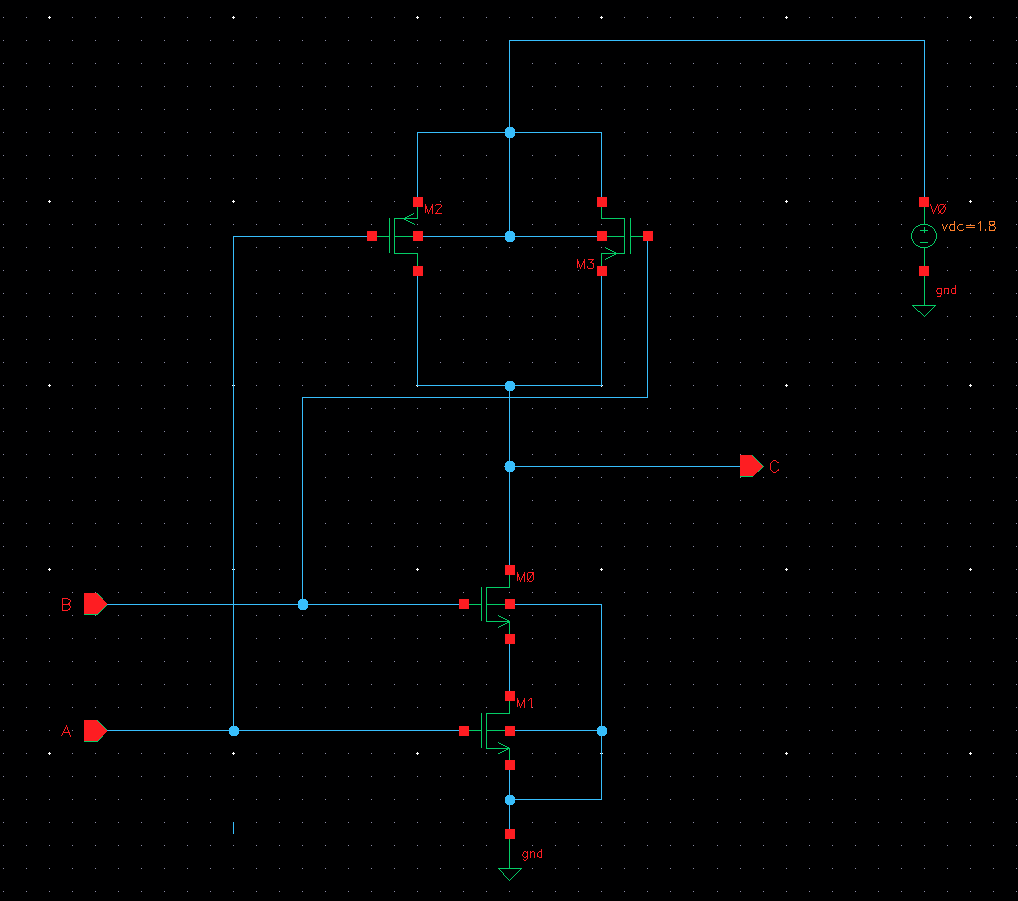
\includegraphics[width=0.7\textwidth]{images/2-input-nand.png}
	\caption{2 Input NAND Gate using CMOS Technology}
	\label{fig:2-input-nand}
\end{figure}

This circuit was then exported as a cellview to be used in the SR latch.

\section{2-Input NOR Gate}
Using basic CMOS implementation, a 2-input NOR gate was designed. The inputs were designated as $A$ and $B$, and the output as $Y$.
\begin{figure}[h!]
	\centering
	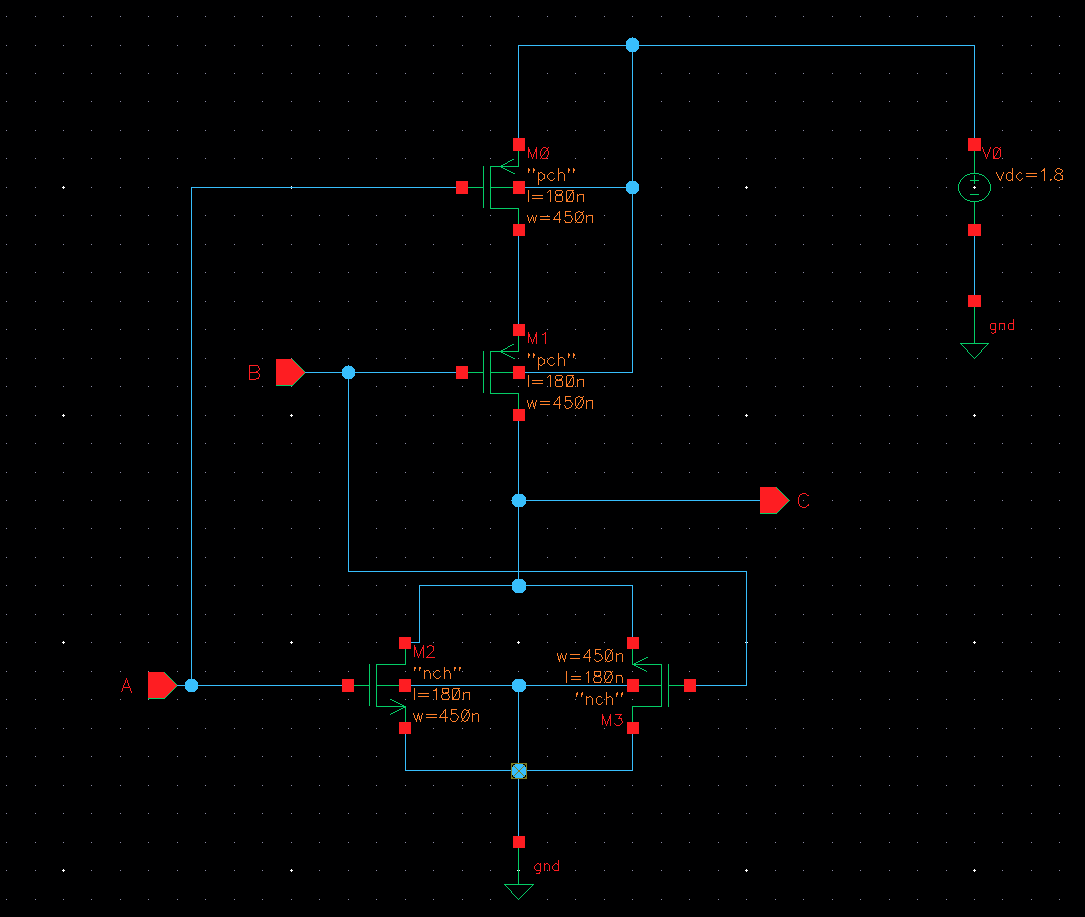
\includegraphics[width=0.7\textwidth]{images/2-input-nor.png}
	\caption{2 Input NOR Gate using CMOS Technology}
	\label{fig:2-input-nor}
\end{figure}

This circuit was then exported as a cellview to be used in the SR latch.

\newpage
\section{SR Latch using NAND Gates}
An SR latch was designed using the previously created 2-input NAND gate cellview. The inputs were designated as $S$ and $R$, and the outputs as $Q$ and $\overline{Q}$.

For brevity's sake, only the NAND implementation is shown, but both the NAND and NOR implementations worked.

\begin{figure}[h!]
	\centering
	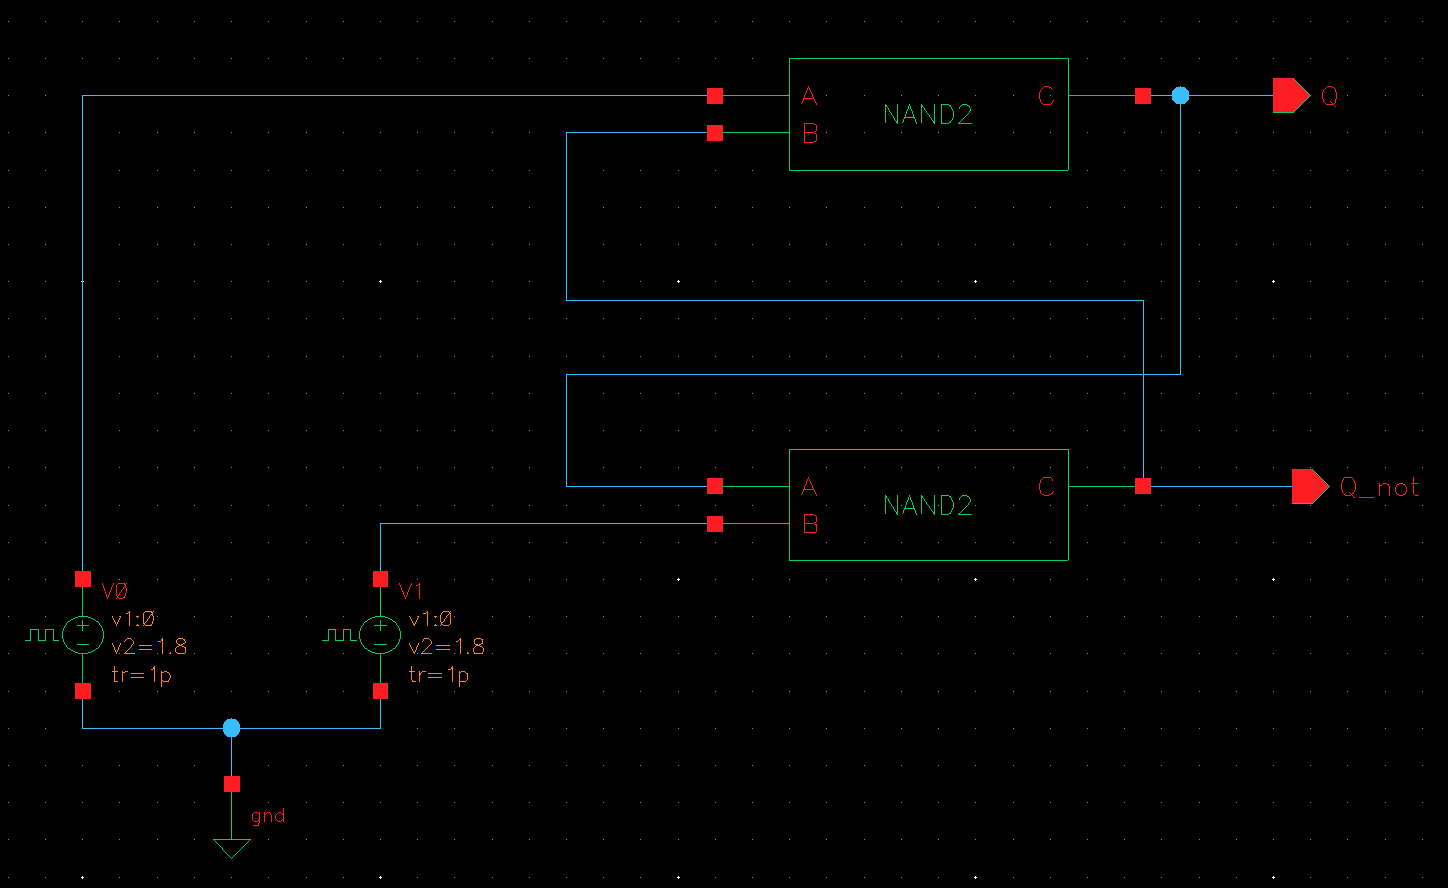
\includegraphics[width=0.7\textwidth]{images/sr-latch-nand.png}
	\caption{SR Latch Circuit using 2-input NAND Gates}
	\label{fig:sr-latch-nand}
\end{figure}

Figure \ref{fig:sr-latch-nand} shows the schematic of the SR latch using NAND gates.

A transient analysis was performed using the oscillating voltage sources shown in Figure \ref{fig:sr-latch-nand} to test the functionality of the SR latch. The results are shown in Figure \ref{fig:sr-latch-nand-waveform}.

\begin{figure}[h!]
	\centering
	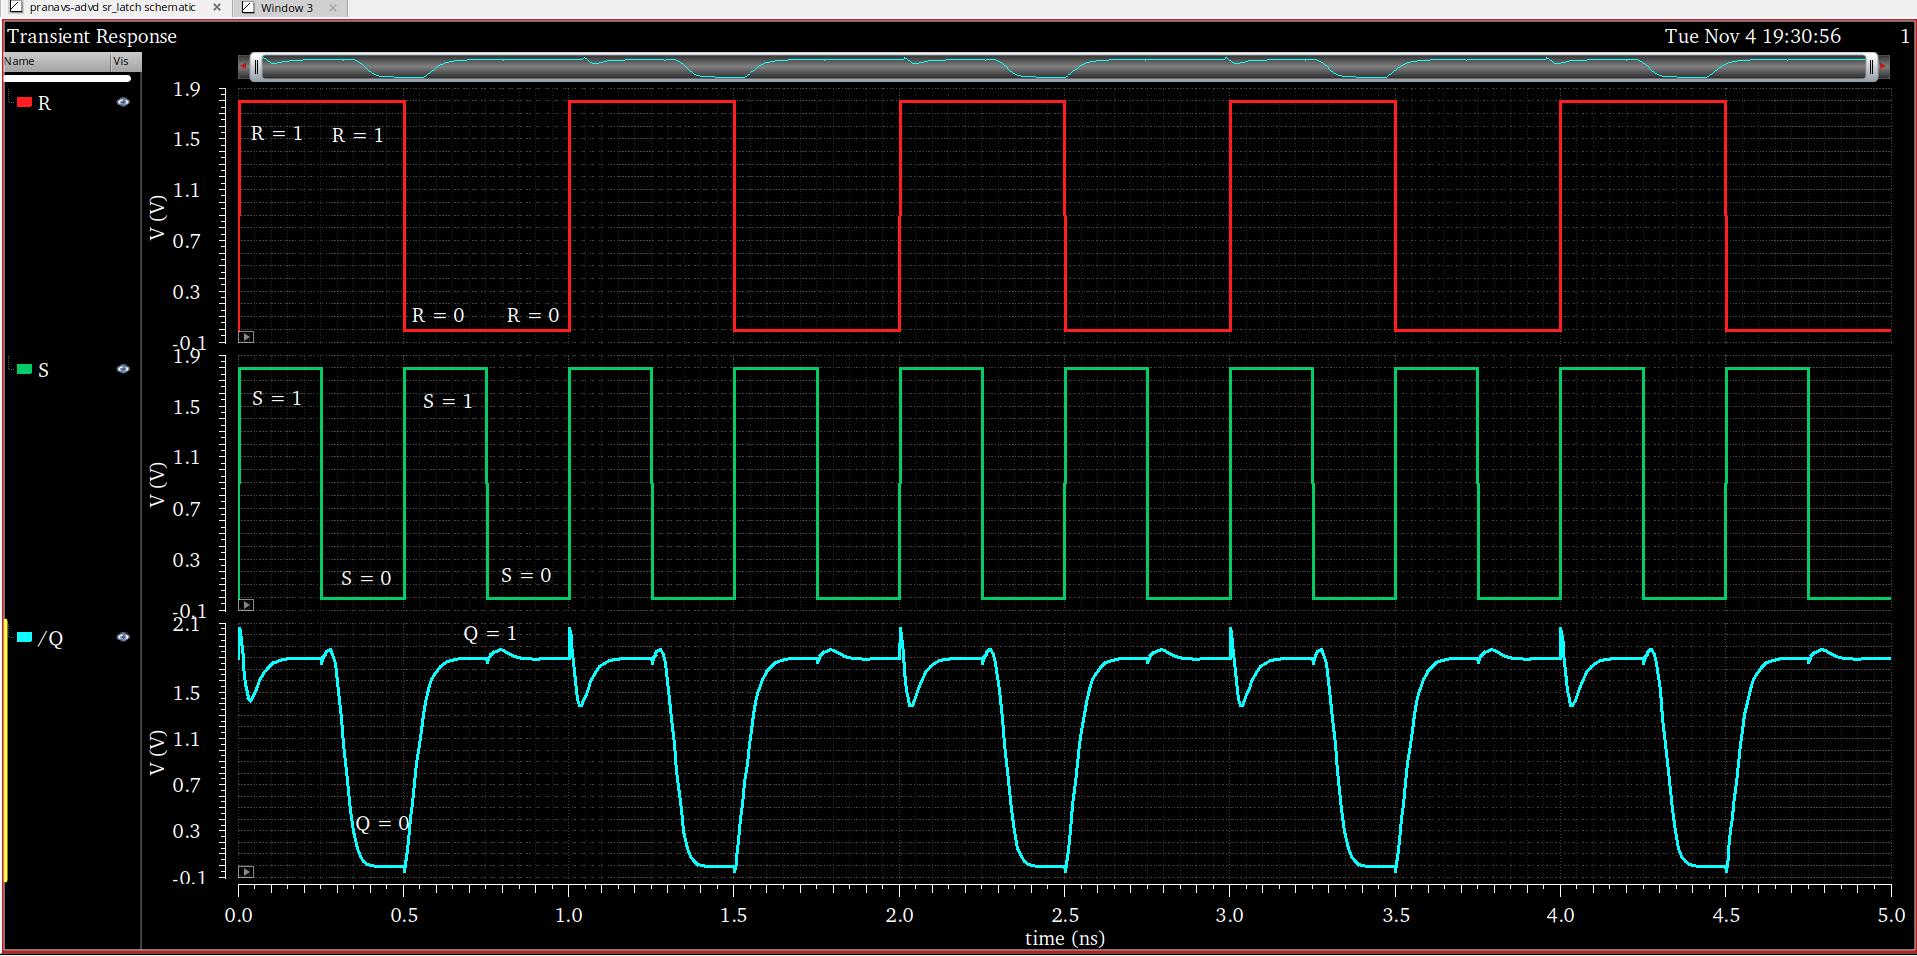
\includegraphics[width=\textwidth]{images/sr-latch-transient.png}
	\caption{Transient Analysis of SR Latch using NAND Gates}
	\label{fig:sr-latch-nand-waveform}
\end{figure}

\end{document}

